% Generated by code/scripts/report_figures.py at 2026-11-03T07:57:50Z; do not edit.
% Inputs: artifacts/local/runs/pipeline-e2e-20261103T075711Z/run
\begin{figure}[t]
\centering
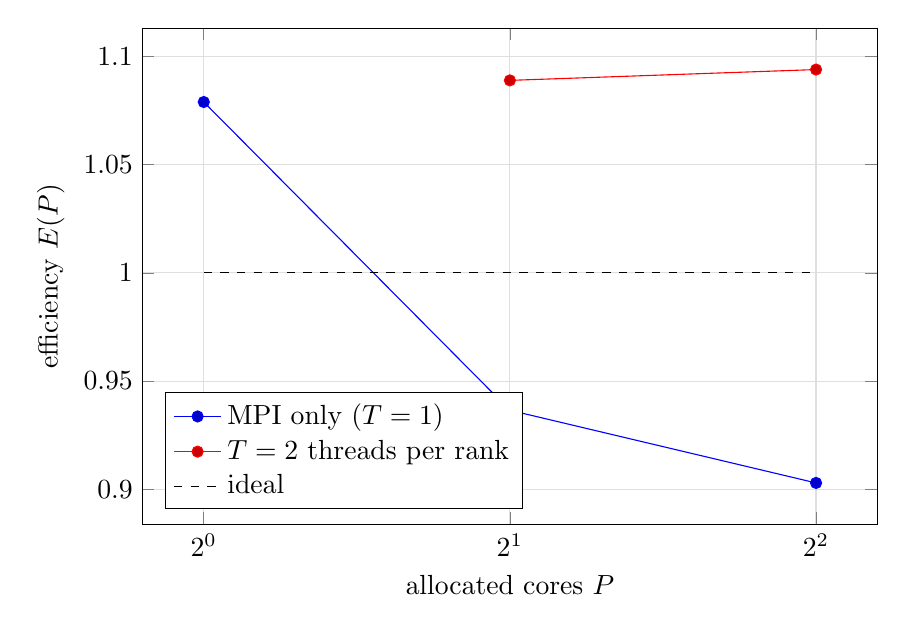
\begin{tikzpicture}
\begin{axis}[width=0.9\columnwidth, height=0.65\columnwidth, xlabel={allocated cores $P$}, ylabel={efficiency $E(P)$}, xmode=log, log basis x=2, legend pos=south west, legend cell align=left, grid=major, grid style={gray!25}]
\addplot+[mark=*] coordinates {(1,1.079) (2,0.9365) (4,0.9029)};
\addlegendentry{MPI only ($T=1$)}
\addplot+[mark=*] coordinates {(2,1.089) (4,1.094)};
\addlegendentry{$T=2$ threads per rank}
\addplot[black, dashed] coordinates {(1,1) (4,1)};
\addlegendentry{ideal}
\end{axis}
\end{tikzpicture}
\caption{\textbf{LOCAL PIPELINE TEST, NOT A MEASUREMENT.} Strong-scaling efficiency. $N=4000$, median of repetitions; serial Barnes--Hut baseline on the same CPU model and build.}
\label{fig:strong-efficiency}
\end{figure}
